\subsubsubsubsection{PrivateMotorVehicle}
\begin{figure}[h]
\centering
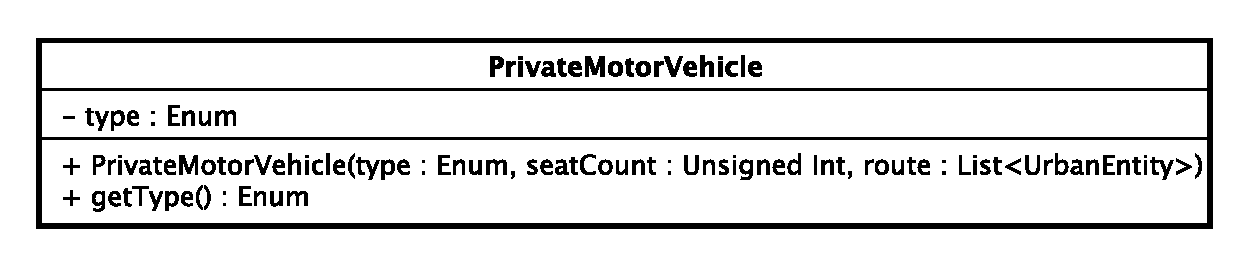
\includegraphics[scale=0.6,keepaspectratio]{images/solution/private_motor_vehicle.eps}
\caption{\pActive::PrivateMotorVehicle}
\label{fig:sd-app-private-motor-vehicle}
\end{figure}
\FloatBarrier
\begin{itemize}
  \item \textbf{\descr} \\
It represents an entity that moves only on roadways.
  \item \textbf{\attrs}
  \begin{itemize}
    \item \texttt{type: Enum} \\
Each vehicle has a type \{ car, motorcycle, sidecar \}.
  \end{itemize}
  \item \textbf{\ops}
  \begin{itemize}
  \item[+] \texttt{PrivateMotorVehicle(type : Enum, seatCount : Unsigned Int, route : List<UrbanEntity>)} \\
Creates a vehicle specifying its type.
    \item[+] \texttt{getType() : Enum} \\
Returns the type of the concrete vehicle.
  \end{itemize}
\end{itemize} 
